\documentclass[journal]{IEEEtran}
\hyphenation{op-tical net-works semi-conduc-tor}

%%%%%%%%%%%%%%%%%%%%%%%%%%%%%%%%%%%%%%%%%%%%%%%%%%%%%%%%%%%%%%%%%%
%%%%%%%%%%%%%%%%%%%%%%%%%%%%%%%%%%%%%%%%%%%%%%%%%%%%%%%%%%%%%%%%%%
%%%%%%%%%%%%%%%%%%%%%%%%% PACKAGES %%%%%%%%%%%%%%%%%%%%%%%%%%%%%%%
%%%%%%%%%%%%%%%%%%%%%%%%%%%%%%%%%%%%%%%%%%%%%%%%%%%%%%%%%%%%%%%%%%
%%%%%%%%%%%%%%%%%%%%%%%%%%%%%%%%%%%%%%%%%%%%%%%%%%%%%%%%%%%%%%%%%%
\usepackage[T1]{fontenc}
\usepackage[utf8]{inputenc}
\usepackage{lmodern}
\usepackage[portuguese]{babel}
\usepackage{graphicx}
\usepackage{fancyhdr}
\usepackage{caption}
\usepackage{subcaption}
\usepackage{placeins}
\pagestyle{fancy}
\usepackage{color}
\newcommand{\HRule}{\rule{\linewidth}{0.5mm}}
\usepackage{listings}
  \lstset{frame=single}
  
  \lstset{language=C++,
                basicstyle=\ttfamily,
                keywordstyle=\color{blue}\ttfamily,
                stringstyle=\color{red}\ttfamily,
                commentstyle=\color{green}\ttfamily,
                morecomment=[l][\color{magenta}]{\#}
}

\begin{document}
\title{ 
Detecção de Objetos Baseada em Subtração de Fundo, Fluxo Óptico e 
Clusterização}
\author{
		Princípios de Visão Computacional - UnB - 2º/2013 \\
		Professor : Flávio Vidal \\
		Aluno : Juarez Aires Sampaio Filho - 11/0032829 \\
		}


\maketitle
\IEEEpeerreviewmaketitle

\section{Objetivos} 
Desenvolver um segmentador de objetos em movimento utilizando para 
isso técnicas de subtração de fundo, fluxo óptico e clusterização.
A aplicação em mente é a detecção de carros em uma câmera de rodovia.
Isto é um teste. Será que vai funcionar?
\section{Introdução}
    Um problema recorrente em visão computacional é 
a segmentação de objetos, isto é, definir quais pixeis de uma
imagem estão associados com objetos. Neste trabalho usamos subtração
de fundo para detecção de objetos em movimentos e um algoritmo baseado
em fluxo ótico e clusterização de pontos para segmentar os diferentes 
objetos. Isto é, não apenas detectamos objetos se movendo, mas 
pretendemos também identificar que esses objetos são diferentes 
entre si.

    A técnica de subtração de fundo consiste em subtrair pixel a 
pixel a imagem atual de uma imagem base considerada como fundo.
O fundo, ou background, é calculado a partir da media dos valores do 
pixel para um número dado de quadros. A técnica é útil para detecção 
de objetos desde que o fundo seja estático, isto é, o fundo e a câmera
estão fixos no tempo. Um dos problemas que surgem na aplicação do 
método é a detecção de sombra, uma vez que o objeto e sua sombra 
podem passar percebidos como um único objeto, sendo que na maioria 
dos casos estamos interessados apenas no objeto em si.

    O fluxo ótico consiste em calcular o campo de velocidade da 
função intensidade de brilho para a cena. O fluxo é calculado de um 
frame para o seu seguinte e nos dá uma informação do movimento que 
ocorre entre os dois quadros. Os princípios do método requerem que a 
luminosidade total da cena se mantenha aproximadamente constante e, 
portanto, grandes variações de brilho são um problema para o método.

    Clusterização consiste em agrupar os dados em diferentes classes. 
O método utilizado é o kmeans, que consiste em minimizar a 
distância entre os pontos e os centros das classes. Essa distância é 
um conceito abstrato e sua definição fica a critério da aplicação.
  
  \newpage
\section{Materiais}
O código elaborado foi feito em C++ as bibliotecas:
\begin{itemize}
    \item core
    \item imgproc
    \item highgui
    \item background\_segm
    \item tracking
\end{itemize}
do \textbf{OpenCV} versão 2.4.6.


\section{Procedimentos}
\subsection{Subtração de Fundo}
Para o cálculo e a subtração de fundo utilizamos a 
classe \textbf{cv::BackgroundSubtractorMOG2} do cabeçalho
\textbf{background\_segm.hpp}. A classe possui métodos para calcular 
o plano de fundo e subtrair este de uma imagem de entrada, obtendo 
assim o primeiro plano, ou foreground. Além disso, a classe já 
implementa um algoritmo de detecção de sombra. O funcionamento dos 
métodos pode ser controlado por meio de parâmetros do objeto. Para 
esse controle foi necessário abrir o .hpp da biblioteca e alterar a 
permissão de acesse dos atributos de controle de private para public.
Seja BGMOG2 um objeto da classe, os principais atributos e métodos 
são:
\begin{itemize}
      \item \textbf{BGMOG2.bShadowDetection } :
      deve ser setado para true para ativar a detecção de sombras
      \item \textbf{BGMOG2.fTau}: controla a 
sensibilidade da detecção de sombras. Se unitário nada é sombra, se 
zero, tudo é sombra. 
      \item \textbf{BGMOG2.operator ()(Mat frame, Mat foreG)}: 
subtrai o fundo de frame e escreve o resultado em foreG, além disso 
atualiza o plano de fundo com informação de frame.
      \item \textbf{BGMOG2.getBackgroundImage(backG)}: retorna o 
plano de fundo.
\end{itemize}

Para a calibração dos parâmetros envolvidos cria-se trackbars para 
controle destes em tempo de execução.

\newpage 
\subsection{Fluxo Óptico}

Para o cálculo do fluxo ótico utilizou-se a rotina \\ 
\textbf{calcOpticalFlowFarneback} do cabeçalho tracking.hpp. A rotina
recebe duas imagens de entrada e escreve em uma de saída o fluxo 
relativo. Além disso outros parâmetros devem ser informados, como o 
critério de fim de parada algoritmo dentre outros. Esse algoritmo 
está na categoria dos algoritmos densos, pois calcula o fluxo para 
todos os pixels da imagem. Para tratamento futuro dos dados, faz-se 
necessário uma filtragem nos dados.

\subsection{Determinando Pontos de Interesse}
Para filtragem dos pontos escolhemos dois critérios:
\begin{itemize}
 \item os pontos pertencem a uma malha quadrada regular de pontos 
igualmente espaçados
  \item o fluxo nos pontos tem um valor mínimo
\end{itemize}
Definimos então um valor de step e varremos o frame de step em step 
adicionando esses pontos e seu respectivo fluxo em um vetor de 
Point's. Depois de selecionados os pontos da malha, varremos estes e 
descartamos aqueles cujo módulo do vetor fluxo correspondente é menor 
que um limiar de threshold. Ao final do processo temos um vetor com 
os pontos de interesse e respectivos fluxos. Esse valor de threshold 
é escolhido em tempo de execução com uma trackbar.

\subsection{Contando o Número de Objetos em Cena}
Para utilizarmos o kmeans precisamos antes determinar o número de 
objetos na cena. Para isso começamos varrendo cada linha daquela 
mesma malha de pontos definida anteriormente e contamos, para cada 
linha, metade do número de vezes que entramos ou saímos em uma região 
onde o módulo do vetor fluxo é maior que o thresohold. A mesma 
varredura é feita no sentido das colunas. A estimação do 
número de objetos é o máximo dessas duas varreduras.

\subsection{Agrupando os pontos de interesse}
Tendo os pontos de interesse e o número de objetos a 
procurar na cena usamos o algoritmo kmeans já implementado na 
biblioteca para agrupar os dados. O algoritmo recebe os pontos a 
serem agrupados, o número de grupos e critérios de parada. No 
trabalho desenvolvido o critério que melhor segmentou os grupos foi a 
posição (x,y) dos pontos de interesse.


\subsection{Calibrando as Constantes}
O uso de trackbars para calibração em tempo de execução 
das constantes resultou nos seguintes parâmetros:
\begin{table}[!htp]
\centering
 \begin{tabular}{|l|l|}\hline
 parâmetro & valor \\ \hline
 detecção de sombra fTau & 0.03 \\ \hline
 threshold de fluxo & 0.05 \\ \hline 
 \end{tabular}
\caption{constantes para os algoritmos}
\label{tab:threshold}
\end{table}


%---------------------------------------------------
%-------------RESULTADOS----------------------------
%--------------------------------------------------
\newpage

\section{Resultados}
A imagens em \ref{fig:resultados} mostram algumas etapas do algoritmo
implementado. Vemos o cálculo do fluxo óptico e a detecção dos objetos para
dois quadros diferentes.


\begin{figure}[h]
  \centering  
    \begin{tabular}{cc}
	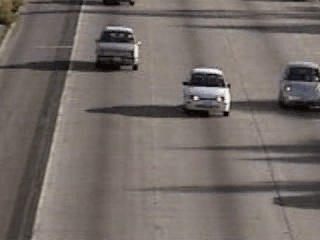
\includegraphics[scale = 0.3]{./images/frame1.jpg}& 
	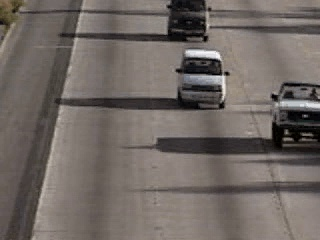
\includegraphics[scale = 0.3]{./images/frame2.jpg} \\
		     \multicolumn{2}{c}{\scriptsize(a) }  \\
	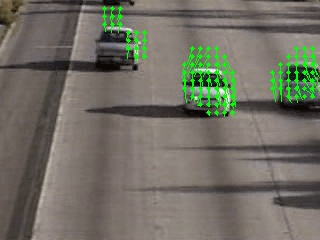
\includegraphics[scale = 0.3]{./images/flux1.jpg} &
	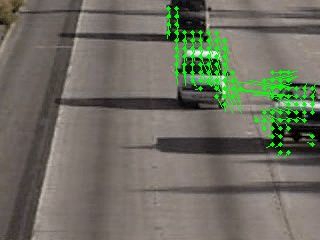
\includegraphics[scale = 0.3]{./images/flux2.jpg}\\
		      \multicolumn{2}{c}{\scriptsize(b) }  \\
	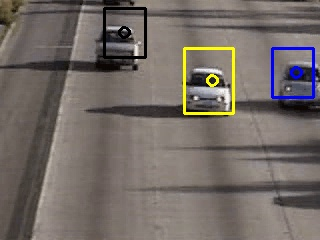
\includegraphics[scale = 0.3]{./images/output1.jpg}& 
	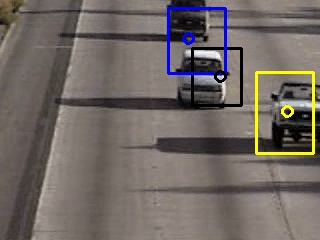
\includegraphics[scale = 0.3]{./images/output2.jpg}\\
		      \multicolumn{2}{c}{\scriptsize(c) }
  \end{tabular}  
  \caption{etapas do processamento para dois instantes : \\
  (a) imagem original,
  (b) fluxo ótico e
  (c) resultado final}
  \label{fig:resultados}
\end{figure}



\section{Resultados}
%---------------------------------------------------
%-------------CONCLUSÃO-----------------------------
%--------------------------------------------------
\newpage
\section{Discussão}
\section{Conclusão}
\begin{thebibliography}{1}

\bibitem{livroPVC}
Forsyth, D.A. , \emph{Computer Vision: a Modern Approach}, 1ªed.

\bibitem{docsOpenCV}
 Documentação do OpenCV, \emph{Tutoriais em Processamento de 
Imagem:Canny Edge Detector, Hough Line Transform e
 Hough Circle Transform}
 Disponível em: http://docs.opencv.org/doc/tutorials/imgproc/table\_of
 
 \_content\_imgproc/table\_of\_content\_imgproc.html
 
 \#table-of-content-imgproc
	 Acesso em 14 de Outubro de 2013.
\end{thebibliography}


\end{document}


